%!TEX root = ../MasterThesis.tex

\section{Peer-to-peer communication}
\label{sec:p2p_communication}

This section explains the core concepts of \gls{P2P} communication technologies. It begins with a comparison of the benefits and disadvantages of centralized and decentralized Web architectures. After that, it shows how \gls{P2P} communication networks can be structured, the different ways to initiate a communication session, as well as how data can be transmitted between peers.

\subsection{Centralized vs. Decentralized Web architectures}
\label{sec:central_decentral_arch}

In classical client-server applications the information is stored on a central system (aka server). Clients have to connect to the server and ask for the information. The server handles the requests from the clients and deliver the information in case a request was valid. Prominent examples of centralized Web architectures are Social Networks such as Facebook or Twitter, in which clients such as a Web browser or Mobile application communicate with a Web service, which runs on a server of the organization providing these Social Networks, to access and retrieve Web documents (e.g.\ \gls{HTML}, images, audio, video, \ldots) via the \gls{HTTP} protocol, as shown in Figure~\ref{fig:p2p_central_server}. \@

\begin{figure}[H]
	\centering
		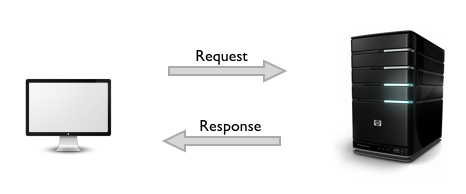
\includegraphics[width=0.9\columnwidth]{images/client-server-web.png}
	\caption[Centralized Web architectures as used by prominent Social Networks]{Centralized Web architectures as used by prominent Social Networks \citep{codeTuts}}
\label{fig:p2p_central_server}
\end{figure}

As a consequence of this architecture all of the information are centralized and under control of the provider of the (Web) service. This can lead to a variety of problems, including serious issues such as unreliable or no longer existing services will result in a dismissal of all the information stored on them, or privacy concerns for user-generated content stored on those central servers. \\

In opposite to that, a \gls{P2P} network considers all nodes as equal. This offers the benefits that information can be kept on each node, and each node can provide access to its information to any other node on the network. Due to this decision, the \gls{P2P} system has an high degree of decentralization, is not owned and controlled by a specific company, and therefore tends to be more resilient to faults, outages and attacks. But due to the distributed nature of it, looking for and accessing information is more difficult. Information in a \gls{P2P} system has to be indexed in a way, so that the correct node is queried for it. Moreover, this index has to be stored somewhere in the system, and the optimal solution for the indexing problem depends on the type of \gls{P2P} system used (see next section). Additionally, the way new nodes get connected to the system is depending on the type of \gls{P2P} system used, and might lead to the introduction of special bootstrap or super nodes into the network as shown in Figure~\ref{fig:p2p_overlay_network} \citep{parameswaran2001p2p}.

\begin{figure}[H]
	\centering
		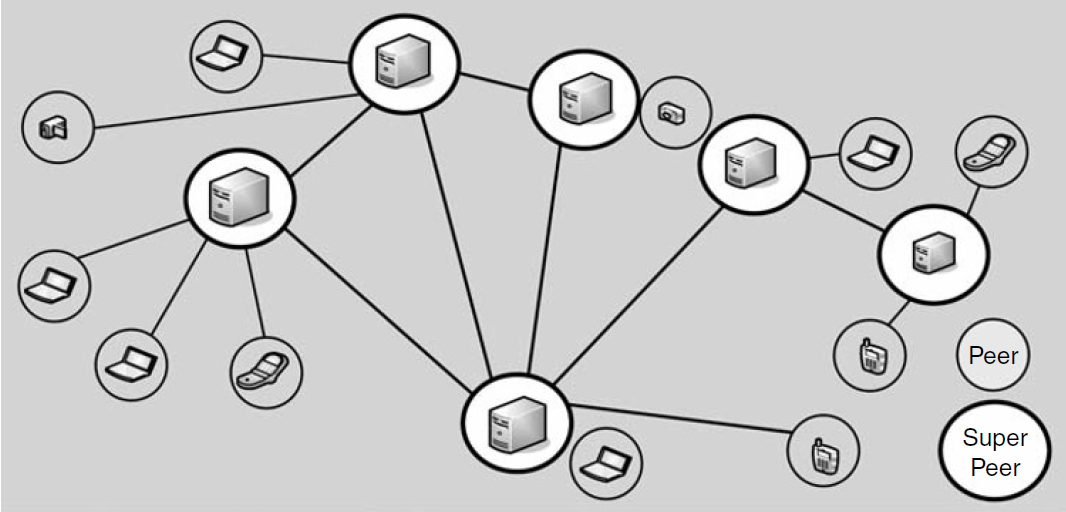
\includegraphics[width=0.8\columnwidth]{images/p2p_network.png}
	\caption[A \gls{P2P} overlay network]{A \gls{P2P} overlay network \citep[pg. 9]{buford2009p2p}}
\label{fig:p2p_overlay_network}
\end{figure}

% section central_decentral_arch (end)

\subsection{Classification of \gls{P2P} systems}
\label{sec:p2p_classification}

\gls{P2P} system architectures can be classified based on their degree of centralization into: \@

\begin{itemize}
	\item \textbf{Partially centralized \gls{P2P} system:} rely on a dedicated controller node that maintains the set of participating nodes, host the index of the information available in the system, and controls the overall operation of the network,
	\item \textbf{Decentralized \gls{P2P} system:} does not use any dedicated controller node, but may need to introduce bootstrap and super nodes for maintaining the list of participating nodes and the index of the information available depending on the size of the network.
\end{itemize}

% section p2p_classification (end)

\subsection{Communication in a \gls{P2P} network}
\label{sec:p2p_start_communication}

\begin{figure}[!ht]
	\centering
	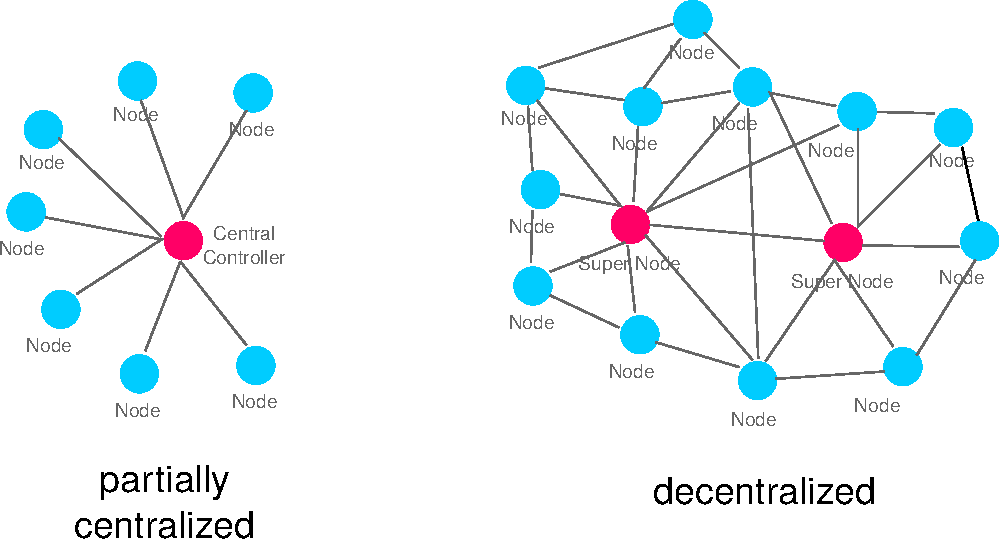
\includegraphics[width=0.8\columnwidth]{images/p2p_network_structures.pdf}
	\caption{Classification of \gls{P2P} networks}
	\label{fig:p2p_network_structures}
\end{figure}

The procedure required to establish a \gls{P2P} communication depends on the structure of the \gls{P2P} system. In a \emph{partly centralized \gls{P2P} system} new nodes join the network by connecting to the central controller first. This central controller has a well-known \gls{IP} address and maintains the operation of the whole \gls{P2P} network. Moreover, any new node has to register with the central controller to get introduced to the \gls{P2P} network. The controller also maintains the information about the overlay network, as well as holds information about each object and on which node(s) it resides within the network. The overlay is typically following a star-shaped topology with the central controller at the centre, see Figure~\ref{fig:p2p_network_structures}. \\

In a \emph{decentralized \gls{P2P} system} new nodes are expected to obtain the \gls{IP} address, which they have to connect to initially, via a separate channel (e.g.\ as a link on a Web site). Depending on the size of the \gls{P2P} network additional bootstrap or super nodes, which help to setup a new node, are available on the network. These special nodes are generally also consolidating information about the objects available on the peers nearby, which helps speeding up searching and accessing required information. The overlay information of such a distributed network can be either \emph{structured}, in which each node receives a unique identifier from a numeric keyspace resembling the responsibilities of that node, or \emph{unstructured}, in which there is no particular network structure, and no further constraints are assigned to the nodes of the network. \\

A \emph{structured overlay} maintain the information within the network more efficiently, because it uses a distributed hash-table to maintain a distributed index, and decides the location (aka node) of an object in the network based on its hash-value. In an \emph{unstructured overlay network} the information is typically stored on the node that introduces it. To locate an object a query request is typically broadcasted through the overlay network. Based on the size of the network and the distance between the node asking for and the node holding the information querying and accessing an information on an unstructured overlay network can take some time, and can also flood the whole network with query requests. Therefore, requesting nodes often set the scope of the request, which limits the number of hops that should be done on the network. This will reduce the communication overhead on the whole system. Additionally, introducing super nodes that collect and maintain indexes of their peers nearby can further reduce the number of hops necessary to find the required information, see Figure~\ref{fig:p2p_network_structures} \citep{rodrigues2010peer}. \@

% section p2p_start_communication

\subsection{The \gls{WebRTC} standard}
\label{sec:p2p_webrtc}

``Web Real-Time Communication (\gls{WebRTC}) is a collection of standards, protocols, and JavaScript \gls{API}s, the combination of which enables peer-to-peer audio, video, and data sharing between browsers (peers)'' \citep[pg. 307]{grigorik2013high}. Although this new \gls{W3C} standard usually stands for in-browser video or audio conferencing without the need of proprietary browser extensions, it also offers ways to exchange arbitrary messages or binary data between participating peers in a distributed Web application. Due to being an open Web standard, \gls{WebRTC} is available in many current Web browsers directly, and is widely adopted as a standardized and open way to establish a \gls{P2P} communication between clients of a Web site, or from within a Web application. The standard wraps a lot of the complexities of establishing peer-to-peer communication channels and transmitting data into three primary \gls{API}s \citep[pg. 307-308]{grigorik2013high}: \@

\begin{itemize}
	\item \textbf{MediaStream:} for acquiring access to and retrieve data from local audio and video devices,
	\item \textbf{RTCPeerConnection:} for establishing a peer-to-peer connection between clients,
	\item \textbf{RTCDataChannel:} for transmitting arbitrary application data
\end{itemize}

To establish a data connection between peers, a Web application has to create a RTCPeerConnection object first, before it can create a RTCDataChannel to exchange messages on it. Establishing a \gls{P2P} connection between globally dispersed peers on the Web is not a trivial task, and has to provide fallback solutions in case of \gls{P2P} connectivity issues due to firewall or \gls{NAT} services used by some of the peers, which usually prevent clients to connect to each other directly. Fortunately, the \gls{W3C} standard is taking care of these steps during the initiating of a \gls{WebRTC} connection by utilizing the \gls{ICE} protocol. After being able to open a connection to another peer, a communication session has to be created. For that, the communicating peers have to negotiate on protocols, encodings, and additional functionality required for the \gls{P2P} communication tasks at hand. The \gls{WebRTC} uses the \gls{SCTP} to exchange application data between peers \citep[pg. 315-330]{grigorik2013high}. It has the following set of features \citep[pg. 342]{grigorik2013high}: \@

\begin{itemize}
		\item \textbf{Reliability:} the data channel can be configured to use either reliable or unreliable delivery of packages,
		\item \textbf{Delivery:} the data channel can be also configured to support either in-order or out-of-order delivery of packages,
		\item \textbf{Transmission:} the transport of data is message-oriented,
		\item \textbf{Confidentiality/Integrity:} all application data transmitted between the peers is encrypted to guarantee confidentiality and integrity of the data exchanged.
\end{itemize}

For a purely data transmission channel one can also disable any audio and video transfers during the setup of the communication session (see Listing~\ref{lst:p2p_webrtc_data_only}). \@

\begin{listing}[H]
	\inputminted[linenos,
							 numbersep=5pt,
							 breaklines=true,
							 frame=lines]{JavaScript}
		{./samples/initiateWebRTCConnection.js}
\caption[Establishing a pure \gls{WebRTC} data connection]{Establishing a pure \gls{WebRTC} data connection \citep[pg. 349]{grigorik2013high}}
\label{lst:p2p_webrtc_data_only}
\end{listing}

Once a data channel has been established between the peers, application data can be exchanged between them via message passing, as shown in Listing~\ref{lst:p2p_webrct_data_send}: \@

\begin{listing}[H]
	\inputminted[linenos,
							 numbersep=5pt,
							 breaklines=true,
							 frame=lines]{JavaScript}
		{./samples/handleWebRTCDataChannel.js}
\caption[Message-oriented communication via a \gls{WebRTC} data channel]{Message-oriented communication via a \gls{WebRTC} data channel \citep[pg. 346]{grigorik2013high}}
\label{lst:p2p_webrct_data_send}
\end{listing}

% section p2p_webrtc (end)

% section p2p_communication (end)
